\documentclass[]{article} % twoside
\usepackage[utf8]{inputenc}
\usepackage[british]{babel}
\usepackage{libertine}
\usepackage[dvipsnames]{xcolor}
\usepackage[a4paper]{geometry}
\usepackage{pdfpages}
\usepackage{parskip}
\usepackage{amsmath, amsthm, amssymb, commath, mathtools}
\usepackage{cancel}
\usepackage{physics}
\usepackage{nicefrac}
\usepackage{booktabs}
\usepackage{tabularx}
\usepackage{upgreek}
\usepackage{tabu}
\usepackage[style=numeric,sorting=none,sortcites=true,backend=biber,natbib=true,language=british,datamodel=software]{biblatex} % sortlocale=de_DE, language=auto, autolang=other
\usepackage{software-biblatex}
\usepackage{enumitem}
\usepackage{graphicx}
\graphicspath{{./plots/}{./images/}}
\usepackage{wrapfig}
\definecolor{capblue}{HTML}{00709B}
\usepackage[margin=1cm,font={small},labelfont={color=capblue}]{caption}
\usepackage{subcaption}
\usepackage{float}
\usepackage{minted}
\usepackage{appendix}
\usepackage{icomma}
\usepackage{multirow}
\usepackage{multicol}
\usepackage[bottom]{footmisc}
\usepackage[separate-uncertainty=true]{siunitx}
\usepackage{tcolorbox}
\usepackage{mhchem}

\usepackage{bbold} % for writing identity

\usepackage[autostyle, english = british]{csquotes} 
\DeclareQuoteStyle[british]{english}% verified
  {\textquotedblleft}
  [\textquotedblleft]
  {\textquotedblright}
  [0.05em]
  {\textquoteleft}
  {\textquoteright} % https://tex.stackexchange.com/q/137210
\MakeOuterQuote{"}
\renewcommand{\ttdefault}{cmtt}

\usepackage{hyperref}
\usepackage{bookmark}
% https://tex.stackexchange.com/a/33701
\makeatletter
    \newcommand{\nonum}[0]{%
        \let\@oldseccntformat\@seccntformat %
        \renewcommand\@seccntformat[1]{}%
        }
    \newcommand{\resnum}[0]{\let\@seccntformat\@oldseccntformat}
    
% for array streching
\renewcommand*\env@matrix[1][\arraystretch]{%
  \edef\arraystretch{#1}%
  \hskip -\arraycolsep
  \let\@ifnextchar\new@ifnextchar
  \array{*\c@MaxMatrixCols c}}
    
\makeatother

\newcommand*{\todo}[1]{\textcolor{red}{TODO: #1}}
\newcommand*{\matrixx}[1]{\underline{\underline{#1}}}
\newcommand*{\vectorx}[1]{\underline{#1}}
\newcommand*{\operatorx}[1]{\hat{#1}}
\newcommand*{\inpycode}[1]{\mintinline{python}{#1}}
\newcommand*{\intermcode}[1]{\mintinline{bash}{#1}}
\newcommand*{\unity}[0]{\mathbb{1}}
\newcommand*{\natzahl}[0]{\mathbb{N}}



\usepackage{chngcntr}
\counterwithin{figure}{section}

\hypersetup{
	pdftitle={NQP Final Programming Exercise},
	pdfauthor={Simon Krumm and Yudong Sun},
	bookmarksnumbered=true,
	bookmarksopen=true,
	bookmarksopenlevel=2,
	pdfstartview=Fit,
	pdfpagemode=UseOutlines,
	colorlinks=true,
	linkcolor=capblue,
	filecolor=magenta,      
	urlcolor=blue,
    citecolor=capblue,
    pdfpagelayout=TwoPageRight
}
\urlstyle{same}

\title{NQP Final Programming Exercise\\-- Exact Diagonalisation --\\{\large [Summer Semester 2023]}}
\author{Simon Krumm and Yudong Sun}
\date{\today}

\addbibresource{sources.bib}

\begin{document}

\maketitle
\section{Introduction}

The problem at hand is to investigate the properties of the ground state of a hardcore-bosonic wheel with different number of lattice sites $L$ on the ring (\autoref{fig:wheel}) using exact diagonalisation (ED) methods. 

\begin{wrapfigure}{r}{0.4\textwidth}
    \centering
    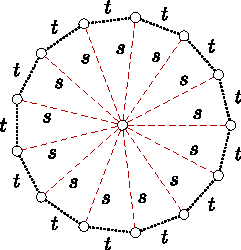
\includegraphics[width=4cm]{graphics/wheel.pdf}
    \caption{Wheel geometry with hopping amplitudes on the ring ($t$) and from the ring to the center ($s$). Illustration from the exercise sheet.}
    \label{fig:wheel}
    \vspace{-1cm}
\end{wrapfigure}

In this problem, two ways to find the ground state (energies) were proposed:
\begin{enumerate}[label=(\roman*)]
    \item The ED of a $(L+1)\times(L+1)$ matrix in the operator-valued vector basis, and
    \item The ED of a $2^{L+1}\times2^{L+1}$ matrix represented in the occupational (Fock) state basis of the tensor-product Hilbert space. 
\end{enumerate}

An immediate consequence that one notices is that the number of eigenvalues obtained for (i) would be significantly less than that from (ii) simply due to the size of the matrix. The discussion of the comparison between these two methods will be carried out in \autoref{sec:c}.

Before we go into the individual problems, we first describe the general structure of the code. The problem-specific implementation in the code shall then be described in the discussion of the problem itself. The programming language of choice was Python. Certain code segments have also been parallelised with \texttt{mpi4py}\footnote{\url{https://mpi4py.readthedocs.io/en/stable/}}, which uses the Message Passing Interface (MPI) under the hood to allow parallelisation across different computing nodes. Unfortunately, the code does not run properly on the cluster for \texttt{nstasks} $> 8$. This problem will be described further under \autoref{sec:parallelisation}. 

The personal desktop PC ultimately used for the generation of this data ran on a 8-core, 16-thread Ryzen 7 5800X, which allowed us to run the calculations with \texttt{nstasks} $= 16$ at higher processor speed ($4.5$ GHz). In the end, the data used for the graphs in this report took approximately 6 hours to generate, before the data was processed and plotted.


\clearpage
\section{Overall Implementation and Code Structure}
    \subsection{Scaffolding}
        The scaffolding of the code is provided by the file \texttt{QM.py}, which contains the following classes:
        \vspace{-0.5\baselineskip}
        \begin{multicols}{2}
            \begin{itemize}
                \item \texttt{State}
                \item \texttt{HBFockState < State}
                \item \texttt{Operator}
                \item \texttt{HBFockOperator < Operator}
            \end{itemize}
        \end{multicols}
        \vspace{-\baselineskip}
        where \texttt{A < B} means that \texttt{A} derives from \texttt{B}, or in other words, \texttt{B} is the parent class of \texttt{A}. \texttt{HBFock} comes from \textit{Hardcore Boson Fock}.
        
        Since operators may be represented by either dense or sparse matrices, this structure allows us to do data-structure agnostic diagonlisaton of the hamiltonians without needing to change large swaths of code. One may choose the representation by passing the parameter \inpycode{sparse = True | False} into the constructor of \inpycode{(HBFock)Operator}. 
        
        Since we are only using states to calculate matrix elements, the time/efficiency benefit of using sparse matrices to represent states are minimal. Therefore, to reduce complexity, all states are represented by dense $(1 \times M)$ or $(M \times 1)$ \texttt{numpy} arrays. 

        All arithmetic operations have also been overloaded such that an expression such as the following becomes possible:
        \begin{align}
            \bra{\varphi} \hat{b}^\dagger \ket{\varphi} \hspace{1cm}\equiv\hspace{1cm} 
            \text{\inpycode{phi.dagger() @ b.dagger() @ phi}}
        \end{align}
        where \texttt{phi} is a \inpycode{State} and \texttt{b} is an \inpycode{Operator}.
        
        Since \texttt{State} also internally stores whether it represents a ket- or a bra-state, the overloaded operations allow us to quickly check if a specific operation is allowed. For example, $\hat{b} \ket{\varphi} \rightarrow \ket{\varphi'}$ and $\bra{\varphi}\hat{b} \rightarrow \bra{\varphi''}$ are allowed but not $\hat{b} \bra{\varphi} \rightarrow~?$. This specifies the expected behaviour of the code and helps us to prevent certain types of errors in the calculations later on that, for example, involve wrong shapes. As a bonus, we will also know the exact datatype of the resulting object after matrix multiplication in normally ambiguous situations:
        \begin{align}
            \braket{\varphi}{\psi} &= (\text{\inpycode{State}})\text{ \inpycode{@} }(\text{\inpycode{State}}) = \text{Number} \\
            \dyad{\varphi}{\psi} &= (\text{\texttt{State}})\text{ \texttt{@} }(\text{\inpycode{State}}) = \text{\inpycode{Operator}}
        \end{align}
        The classes \inpycode{HBFockState} and \inpycode{HBFockOperator} are then a specific implementation of \inpycode{State} and \inpycode{Operator} respectively for the problem at hand. They contain checks for shape requirements and stores additional parameters relevant for the calculation. Furthermore,  \inpycode{HBFockOperator} provides a method for expanding single site ($\tilde{L} = 0$, "only center site") operators to the many-body ($\tilde{L} = L)$ Hilbert space. There, we make use of the fact that the tensor product of identity matrices is simply a larger identity matrix ($\unity{}^{\otimes n}_2 = \unity_{2^n}$) to simplify the calculations and reduce overhead. 

        Where possible, robust type-hinting has also been added to the code. This way, code could be more easily be verfied, and it would be easier for another person to follow the logic in the code. 

    \subsection{Main Code}
        The main code that does the calculation is contained in \texttt{src/main.py} in the form of a \inpycode{Lattice} class and the function \inpycode{condensate_frac()}.

        The \inpycode{Lattice} class provides the wrapper for a wheel lattice with a given number of lattice sites $L$ in the ring. It contains the methods for building the Hamiltonian in the following bases:
        \begin{itemize}
            \item Operator-valued vector basis (\autoref{sec:a}, Problem 1(a)): 

            $\text{\inpycode{lattice.build_hamiltonian_manual(t, s)}} \rightarrow \matrixx{H}_\odot = \text{\inpycode{lattice.hamiltonian["manual"]}}$
            
            \item Fock state basis of the tensor-product Hilbert space (\autoref{sec:b}, Problem 1(b)): 
            
            $\text{\inpycode{lattice.build_hamiltonian_ed(t, s)}} \rightarrow \operatorx{H}_\odot = \text{\inpycode{lattice.hamiltonian["exact"]}}$
        \end{itemize}

        To obtain the spectrum as a function of the relative coupling $s/t$, we use the function \inpycode{spectrum(type_)}, where \inpycode{type_ = "exact" | "manual" }. In this case, it makes sense to set $t = 1$ and then simply loop over $s/t$  values (\inpycode{s_t[]}), i.e. $s$ is in units of $t$. In each step, we build the Hamiltonian$$\text{\inpycode{lattice.build_hamiltonian_*(t = 1, s = s_t[i])}}$$ and calculate the desired eigenvalues using the helper functions provided by the \inpycode{(HBFock)Operator}. The eigenvalues are then saved as a CSV file.

        Here, when instantiating the \inpycode{Lattice} class, we have the choice of representing the Hamiltonians either as sparse or dense matrices. While using sparse matrices may be faster, we are unable to extract all the eigenvalues of the matrix due to the ARPACK implementation of the eigensolver \cite{lehoucqARPACKUsersGuide1997}. As a result, we only extract the $N-1$ largest eigenvalues (in terms of magnitude, i.e. $-1 > 0.5$) of the $N \times N$ matrix, which should be sufficient for our purposes. This corresponds to the mode \texttt{LM} in \texttt{scipy.linalg.sparse}'s eigenvalue function(s). To extract all the eigenvalues, packages such as FILTLAN \cite{fangFilteredLanczosProcedure2012} could be used instead.

        For each given $L$, the condensate fraction is then calculated using the \inpycode{condensate_frac()} function. Initially, this particular function was separated out from the \inpycode{Lattice} class as it looped over a sequence of $L$'s, $L \in \natzahl$, $L \geq 2$, and calculated the condensate fraction for each $L$. However, we realized that since we did not know how long each iteration would take, it would make more sense for \inpycode{condensate_frac()} to calculate each $L$ separately and save the intermediate data. This way, we could interrupt the running code at any time and retain the results that have already been calculated. Due to time constraints, this function was not rewritten to be a part of the \inpycode{Lattice} class.

        For the calculation of the condensate fraction, using sparse matrices resulted in some artefacts in the results. We thus decided to only use dense matrices for the calculation in problem 1(d) (\autoref{sec:d}). 

        % np.power(10, np.linspace(start=-2, stop=1, num=112))
        In our final implementation, we used $S = 112$ equidistant samples between $s/t = 10^{-2}$ and $s/t = 10^{1}$ on the logarithmic scale to calculate the spectrum as a function of the relative coupling, and we used $S = 256$ equidistant samples between $s/t = 10^{-3}$ and $s/t = 10^{3}$ on the logarithmic scale to calculate the condensate fraction. 

    \subsection{Parallelisation}
        \label{sec:parallelisation}
        As an embarrassingly (or pleasingly) parallel task, the calculation of the eigensystem for different $s/t$ values was parallelized with the help of \texttt{mpi4py}. In this case, our \inpycode{s_t[]} array was split into \texttt{NTasks} equal chucks and then distributed. Each node then did its own calculation for its own set of $s/t$ values before all the results are gathered again back to the root node. 

        The root node then does the rest of the processing before saving the results into a CSV file. 

        Initially, a contingent of \texttt{NTasks} $ = 50$ using the \texttt{cip} cluster was planned. However, we kept encountering the following error:
        \begin{minted}[breaklines,autogobble,frame=leftline,framesep=10pt]{text}
        srun: fatal: SLURM_MEM_PER_CPU, SLURM_MEM_PER_GPU, SLURM_MEM_PER_NODE are mutually exclusive
        \end{minted}
        which we were unable to resolve on our end. We postulate that if we managed to be lucky enough for the job to be assigned to a single computing node, this problem would resolve itself. This was however difficult to test with \texttt{NTasks} $ = 50$, since every time we requested a job, it ran across multiple nodes. There was just one MPI successful run on the cluster with \texttt{NTasks} $ = 8$ and explicitly requesting for \texttt{cip-cl-compute7}. This job managed to calculate the condensation fraction for $L = 2$ to $L = 10$ in a little over 2 hours\footnote{The job script for this job is available under \texttt{src/run\_cluster\_mpi.sh}.}. In comparison, it took about approximately 30 minutes on our local desktop machine with \texttt{NTASKS} $= 16$.
        
        We therefore came to the conclusion that while we could reduce \texttt{NTASKS} for running on the cluster, the cluster does not actually offer any benefits over using our own desktop PC. It was decided that the parallelised code will then be run on a local desktop PC instead of the cluster. For use on the cluster, it is recommended to just run the "single thread" version without parallelisation using MPI.
    
    \subsection{Running the code}

        The code is strictly split into data acquisition and data processing. The data acquisition is covered in \texttt{src/main.py}, which is separately controlled by \texttt{src/run.py} and \texttt{src/run\_cluster.py}. The latter is meant to run the data acquisition on the cluster, while the first was designed to run the data acquisition on a private desktop. This decision was made due to the problems with running the MPI parallelization on the cluster as explained in the section \ref{sec:parallelisation} above. 

        Running the data acquisition with or without MPI amounts to passing \inpycode{mpi = True | False} to the \texttt{Lattice} class or the \inpycode{condensate_frac()} function. 

        The data is then stored in separate \text{.csv} files in the data folder and manually moved to new subfolders to differentiate between runs. 

        There is no need for manual interaction with \texttt{main.py}, only with the file \texttt{run.py} should be used to adjust which data to gather and for which $L$'s. This is exemplified in the snippet below for a full MPI data acquisition run on a local desktop. (via \texttt{run.py})

        \begin{minted}
        [linenos,breaklines,autogobble,frame=leftline,framesep=10pt]{bash}
        for L in range(2,12):
            lattice = Lattice(L, "sparse", mpi = True)
            lattice.spectrum("manual")
            lattice.spectrum("exact")
            condensate_frac(L, matrix_type = "dense", mpi = True)
        \end{minted}

        Running the file with MPI amounts to calling \intermcode{mpiexec -n $NUM_NODES python3 run.py}, where \texttt{run.py} can be called in the usual way for a non MPI run (note that the arguments in \texttt{run.py} need to be adjusted).

        The data processing is purely based on the \texttt{data\_processing.py} file, which includes three functions, \inpycode{plot_manual()}, \inpycode{plot_exact()} and \inpycode{plot_cf()}. These take care of the plots for Problems a), c) and d) in order, i.e. running the data processing file as provided below will evaluate all data.

        \begin{minted}[linenos,breaklines,autogobble,frame=leftline,framesep=10pt]{bash}
        if __name__ == "__main__":
            plot_manual()
            plot_exact(manual_subset = False)
            plot_exact(manual_subset = True)
            plt_cf()
        \end{minted}

        The first two functions will create a plot each in the plots folder that contains 10 subplots, for system sizes ranging from $L=2$ to $L=11$. The last function will create a plot with two subplots that show the condensation fraction separately for even and odd $L$. 

        The argument \inpycode{manual_subset} processes the same data if set to \inpycode{True}, but only plots the first 2 subplots. This is favorable because the range of the data for $L = 2$ and $L=3$ are much smaller than that of larger system sizes. This affords a better resolution to the plot.

        Therefore, the only manual interaction with the \texttt{data\_processing.py} file needed is the modification of the filepaths to change which folders are targeted to draw data from.

        \texttt{python3 data\_processing.py} can be called in the usual way since there is no MPI interaction from this point on.

    \subsection{Runtimes}
        Since running MPI parallelised on the cluster did not work, the fastest runtime was achieved on a private desktop. Naturally, the data acquisition is the crucial step in terms of runtime.

        For the largest $L=11$ ($12$ lattice sites) run, the full runtime for data acquisition amounted to about $6$ hours, where $5$ of those were dedicated to the $L=11$ case. Our estimations put the $L=12$ case to add another $35-40$ hours to this, making this an unreasonable goal for a non-parallelised cluster run.
        
%     TODOs:
% \begin{itemize}
%     \item Bundles observation, eigenvalue crossings -> Limitation
%     % \item Structure of the code
%     % \item MPI/Parallelization
%     % \item implementation of sparse matrices
%     \item interpretation of (d)
%     \item How we obtained the data, and how long the run took with MPI
%     % \item Tests for expanding and fock
%     \item verbessung -> Jordon Wigner transformation
%     \item Uncomment the run.py
%     \item make a cluster run.py
%     \item last step took 4 hrs, would not be able to complete
% \end{itemize}
\clearpage
\section{Problem 1}

\subsection{Problem 1 (a)}
    \label{sec:a}
    The matrix form of this Hamiltonian can be obtained by comparing explicitly in calculation
    
    \begin{align}
        &\begin{pmatrix}[1.5]
            b^\dagger_0 & b^\dagger_1 & \hdots & b^\dagger_{L-1} & b^\dagger_\odot
        \end{pmatrix}
        \begin{pmatrix}[1.5]
            M_{0,0} & M_{0,1} & \hdots & M_{0,L-1} & M_{0,L} \\
            M_{1,0} & M_{1,1} & \hdots & M_{1,L-1} & M_{1,L} \\
            \vdots & \vdots & \ddots & \vdots & \vdots \\
            M_{L-1,0} & M_{L-1,1} & \hdots & M_{L-1,L-1} & M_{L-1,L} \\
            M_{L,0} & M_{L,1} & \hdots & M_{L,L-1} & M_{L,L}
        \end{pmatrix}
        \begin{pmatrix}[1.5]
            b^\dagger_0 \\ b^\dagger_1 \\ \vdots \\ b^\dagger_{L-1} \\ b^\dagger_{\odot}
        \end{pmatrix} \\
        & = \underbrace{\sum_{i=0}^{L-1} b^\dagger_i M_{ii} b_i}_\text{diagonal} + \underbrace{\sum_{i\neq j}^{L-2} b^\dagger_iM_{ij}b_j}_\text{rest} + \underbrace{\sum_{i=0}^{L-2} b^\dagger_iM_{iL}b_\odot}_\text{rightmost col \textbackslash diag} + \underbrace{\sum_{i=0}^{L-2} b^\dagger_\odot M_{Li}b_i}_\text{bot row \textbackslash diag}
    \end{align}
    
    Since the operators on different sites commute, the matrix entries can be read off the Hamiltonian as 
    \begin{align}
        \begin{pmatrix}[1.3]
            0 & -t & \hdots & -t & -s \\
            -t & 0 & \hdots & -t & -s \\
            \vdots & \vdots & \ddots & \vdots & \vdots \\
            -t & -t & \hdots & 0 & -s \\
            -s & -s & \hdots & -s & 0
        \end{pmatrix}
    \end{align}
    This $(L+1) \times (L+1)$ matrix is diagonalised for a sample of values of $\nicefrac{s}{t}$. As previously mentioned in the implementation section, this is done by setting $t=1$ and varying $s$, which can be interpreted as expressing the center hopping strength s in units of on-wheel hopping strength $t$. We obtain a set of eigenvalues for each hopping strength $s$. The eigenvalues are sorted by magnitude and plotted. The largest and smallest eigenvalue are always coloured individually, all others have the same colour. \autoref{fig:spectrum_manual} shows the log-linear plot for $L = 2$ up to $11$, corresponding to $12$ sites in total with the center.

    The first observation is the fact that all plots are similar. While the number of eigenvalues increases, there are only three distinct "trajectories": the first and last eigenvalue split up, while all other eigenvalues are constant on a line. When the last eigenvalue and the constant eigenvalues cross, the colours swap since the eigenvalues are ordered by magnitude. 
    
    Theoretically, it could be possible to keep track of the eigenvalues correctly by calculating the derivatives at the crossing to identify each eigenvalue. However, it was not immediately clear to us how to do that and so we decided against doing it due to time constraints. 
    
    The most important feature is that the splitting increases in magnitude as the number of sites go up. One minor observation is the fact that the first and last eigenvalues start out symmetrically spaced around 0 for $L=2$, but the ground state drops with increasing $L$ right from the smallest $\nicefrac{s}{t}$ value. 
    
    In short, as $L$ increases, the split off of the ground state increases and the initial ground state energy decreases.

    \begin{figure}[!t]
        \centering
        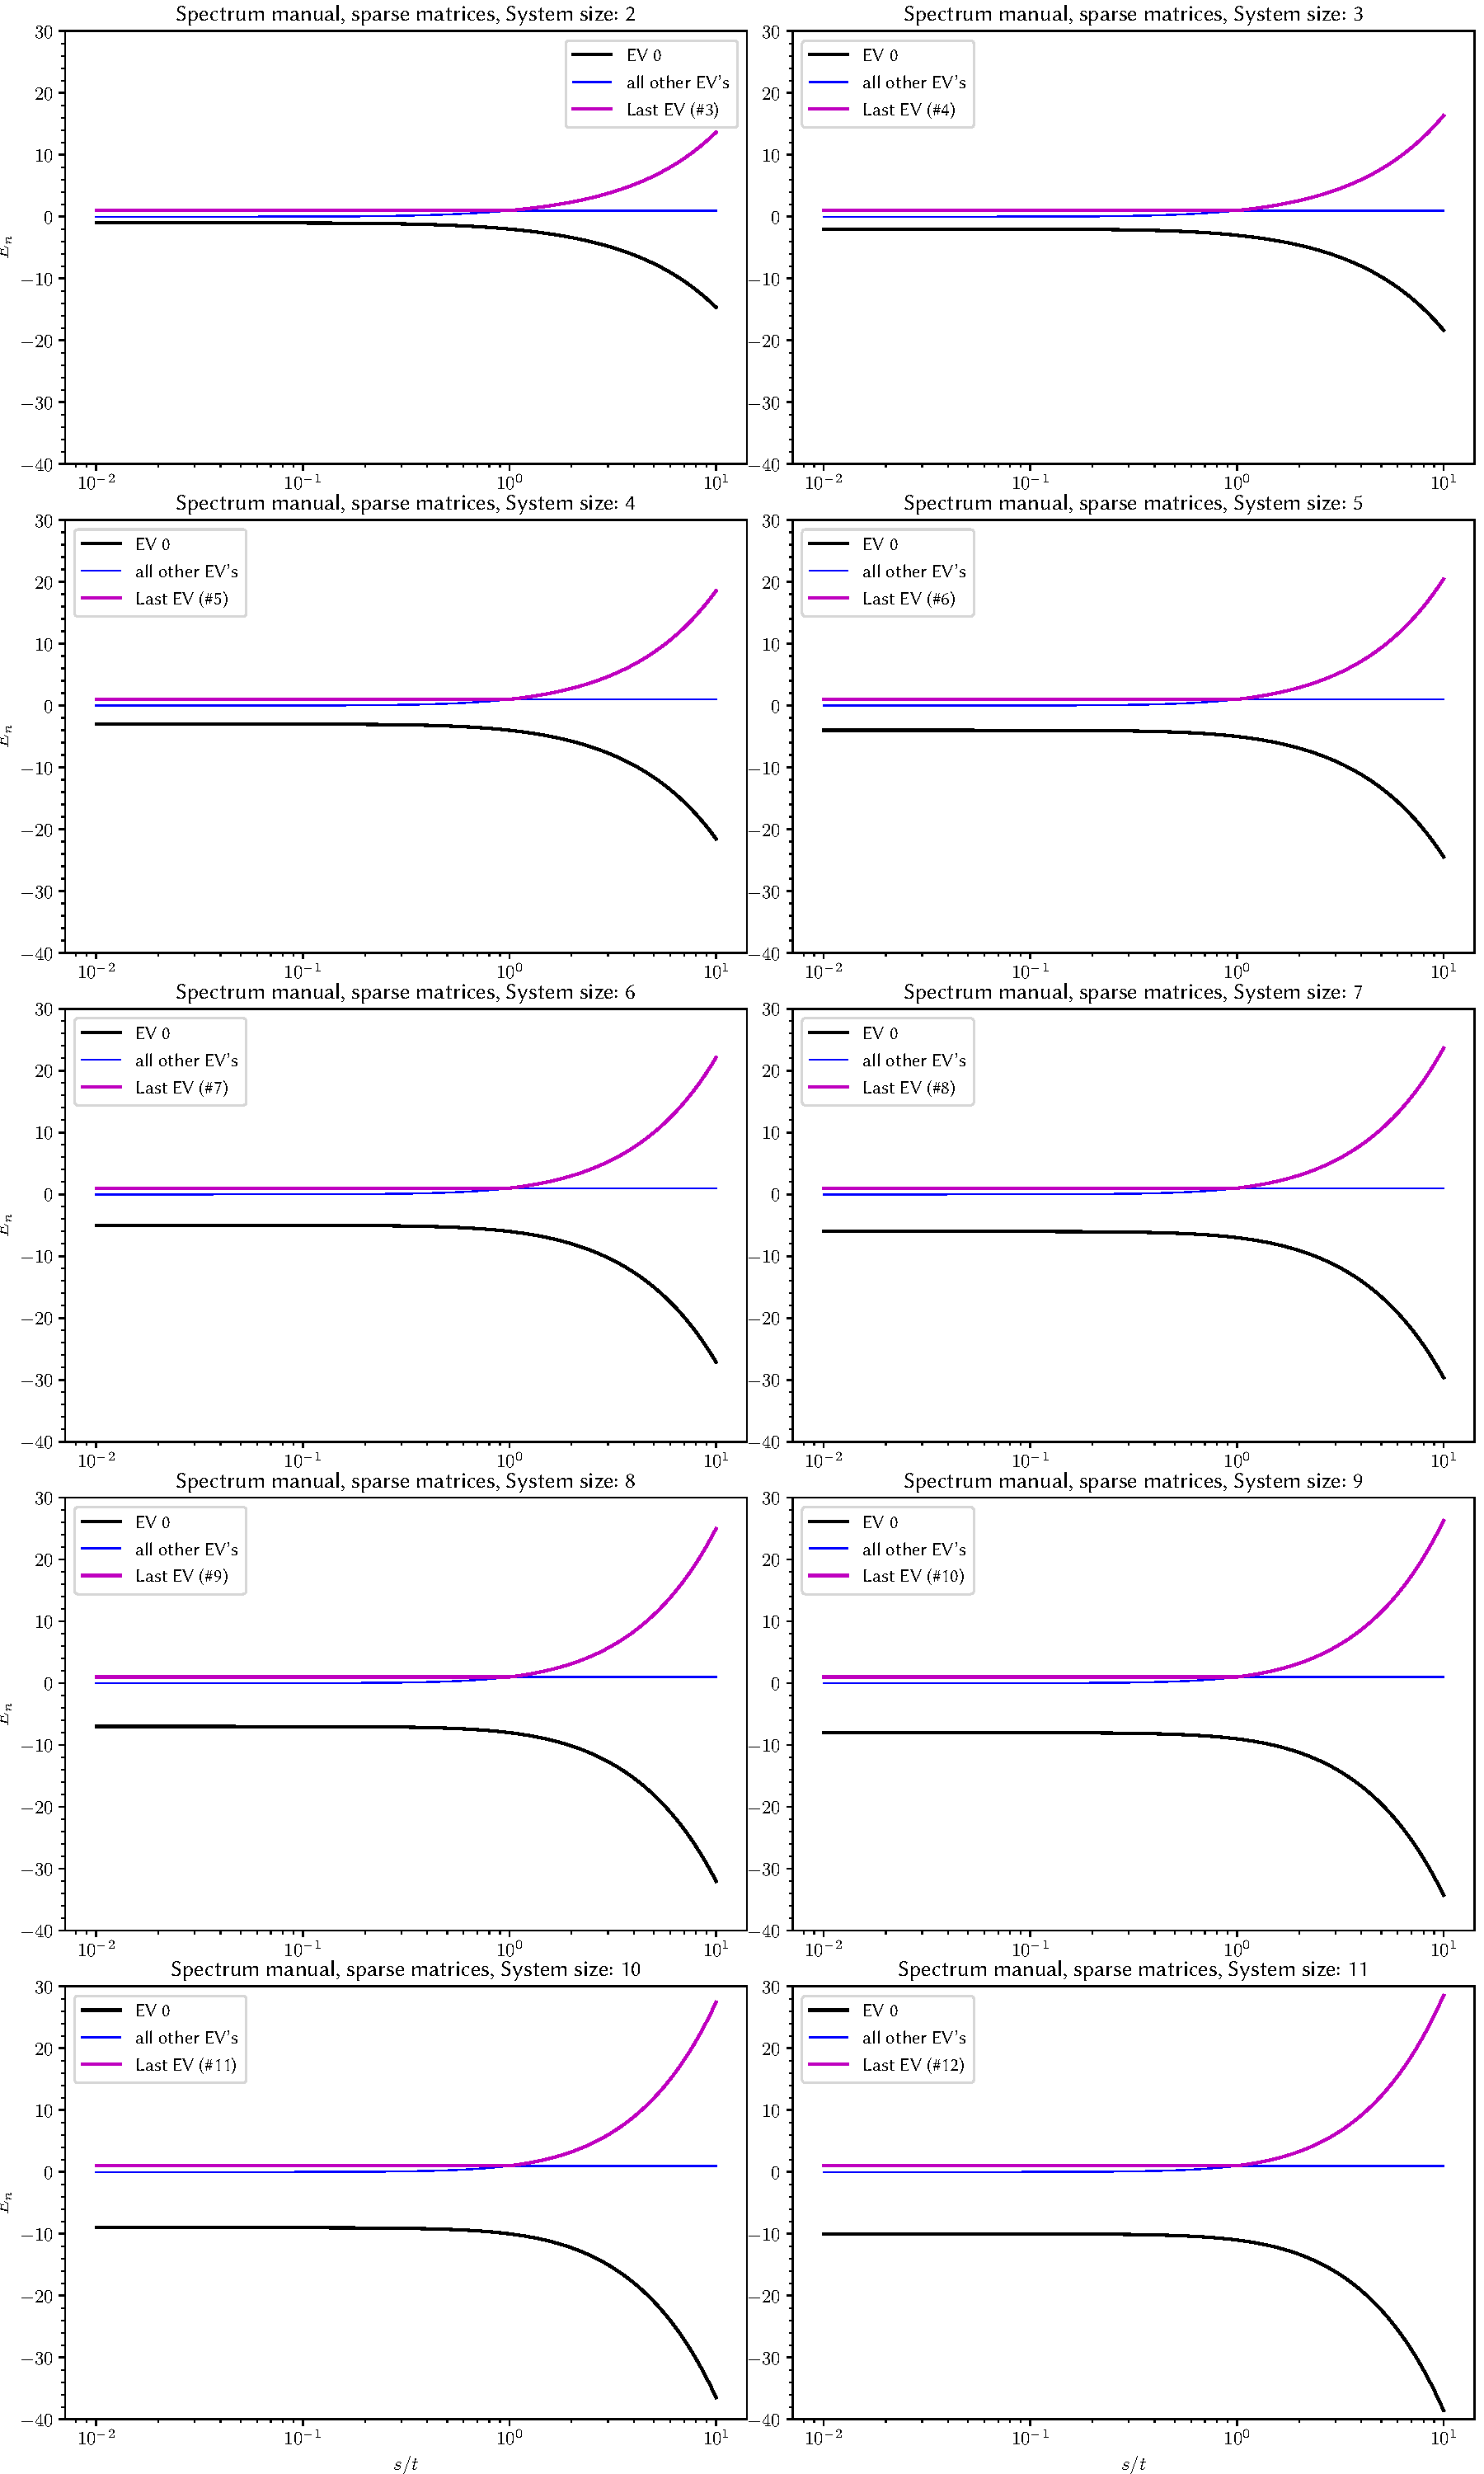
\includegraphics[width=\textwidth]{graphics/spectrum_manual.pdf}
        \caption{Spectrum of singe-particle Hamiltonian for different system sizes}
        \label{fig:spectrum_manual}
    \end{figure}
    \clearpage

\subsection{Problem 1 (b)}
    \label{sec:b}
    It is simple to check that the following identifications from  \cite{Streib} satisfies the commutation relations proposed in the problem statement:
    \begin{align}
        \hat{h_i} = \hat{S}^+_i \hspace{20pt} \hat{h_i}^\dagger = \hat{S}^-_i \hspace{20pt} \hat{S}^\pm_i = \hat{\sigma}^x_i\pm\hat{\sigma}^y_i \hspace{20pt} i \in \{1, ..., L\}
    \end{align}
    We map an "empty site" to $[1, 0] =: \ket{\uparrow}$ and an "occupied site" to $[0, 1] =: \ket{\downarrow}$. The hardcore bosonic ladder operators can then be represented in the Fock basis, e.g. for four sites, $\ket{0011} \hat{=} \ket{\uparrow} \otimes \ket{\uparrow} \otimes \ket{\downarrow} \otimes \ket{\downarrow}$. This fixes the representation of the hardcore bosonic ladder operators in the Fock basis to 
    \begin{align}
        \hat{h_i} = \hat{S}^+_i = \underbrace{\unity \otimes \unity \otimes \dotsm}_\text{i times} \otimes~\hat{S}^+ \otimes \underbrace{\dotsm \otimes \unity \otimes \unity}_\text{L-i times}
    \end{align}
    With this mapping, the Hamiltonian comes out to be a $2^{L+1} \times 2^{L+1}$ matrix. The correlator matrix takes the same size and can easily be assembled from the hardcore bosonic operators.

\subsection{Problem 1 (c)}
    \label{sec:c}
    This matrix is diagonalised for $\nicefrac{s}{t}$ values just like for Problem 1(a) (\autoref{sec:a}). The plot with the eigenvalues for up to $L=11$ is depicted in  \autoref{fig:spectrum_exact}. The first two plots are also shown magnified in \autoref{fig:spectrum_exact_subset}.
    
    The first and last eigenvalues are initially colored differently again, but they are quickly overtaken by the huge bundle of intermediate eigenvalues, which splits up into 3 major branches. Just like before, the color mapping fails at the crossings, resulting in a kink, because it was too difficult to keep track of the numerous eigenvalues (! $4095$ at $L=11$) and their derivatives on the plot. The plot essentially shows the same characteristic as the one in \autoref{fig:spectrum_manual}, with the main difference being the number of Eigenvalues and the spread. The eigenvalues start out constant as well, but additional intermediate eigenvalues start out anywhere between the first and last. Additionally, some of the intermediate eigenvalues also split up and down, essentially forming 3 bundles of eigenvalues. The spread of the bundles increases with the number of sites, and the ground state energy drops for all values of $\nicefrac{s}{t}$. For $L=11$, the plot becomes so crowded that even at negligible plotting linewidth, the bundles merge into one.
    
    \begin{figure}[b!]
        \centering
        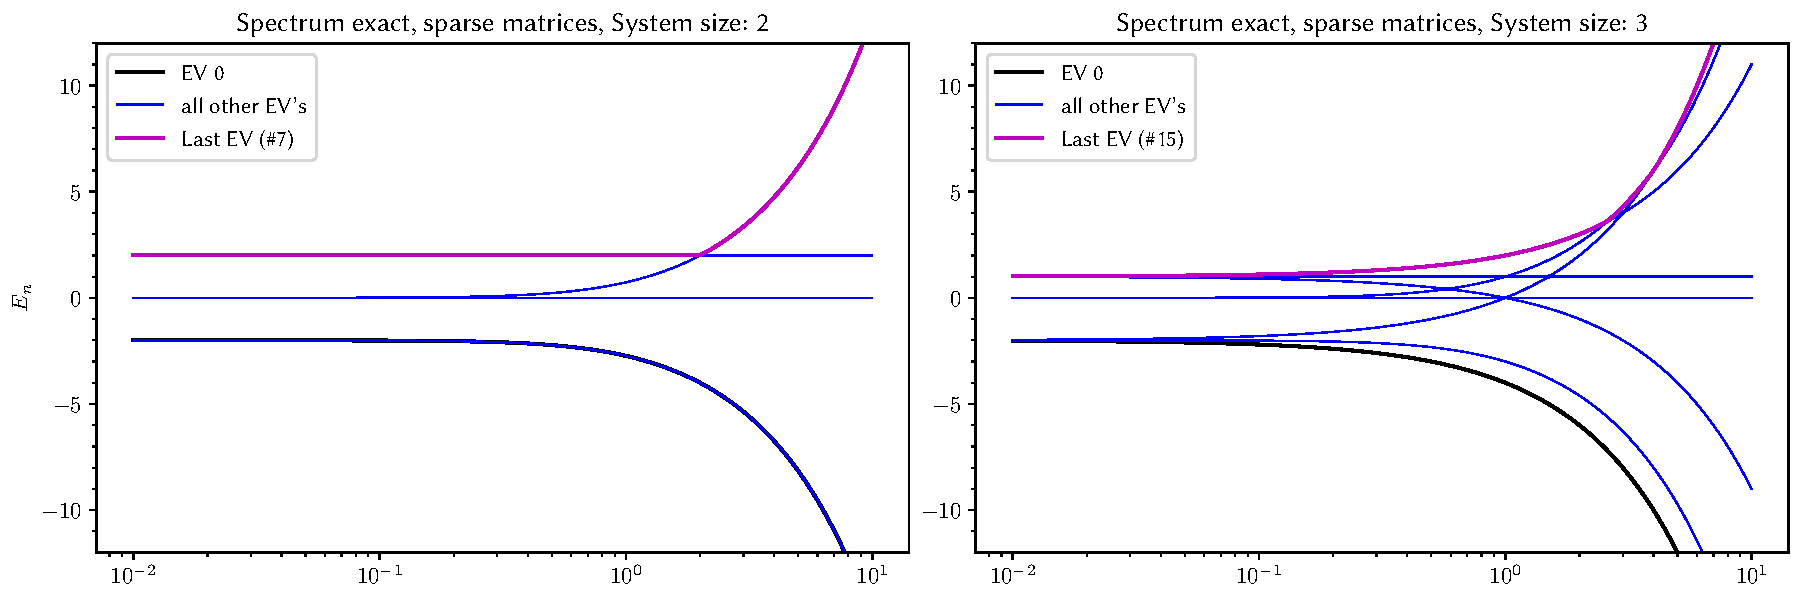
\includegraphics[width=\textwidth]{graphics/spectrum_exact_manual_subset.pdf}
        \caption{Spectrum of Hamiltonian for $L = 2, 3$, which are the first two subplots of \autoref{fig:spectrum_exact}.}
        \label{fig:spectrum_exact_subset}
    \end{figure}

    \begin{figure}[t!]
        \centering
        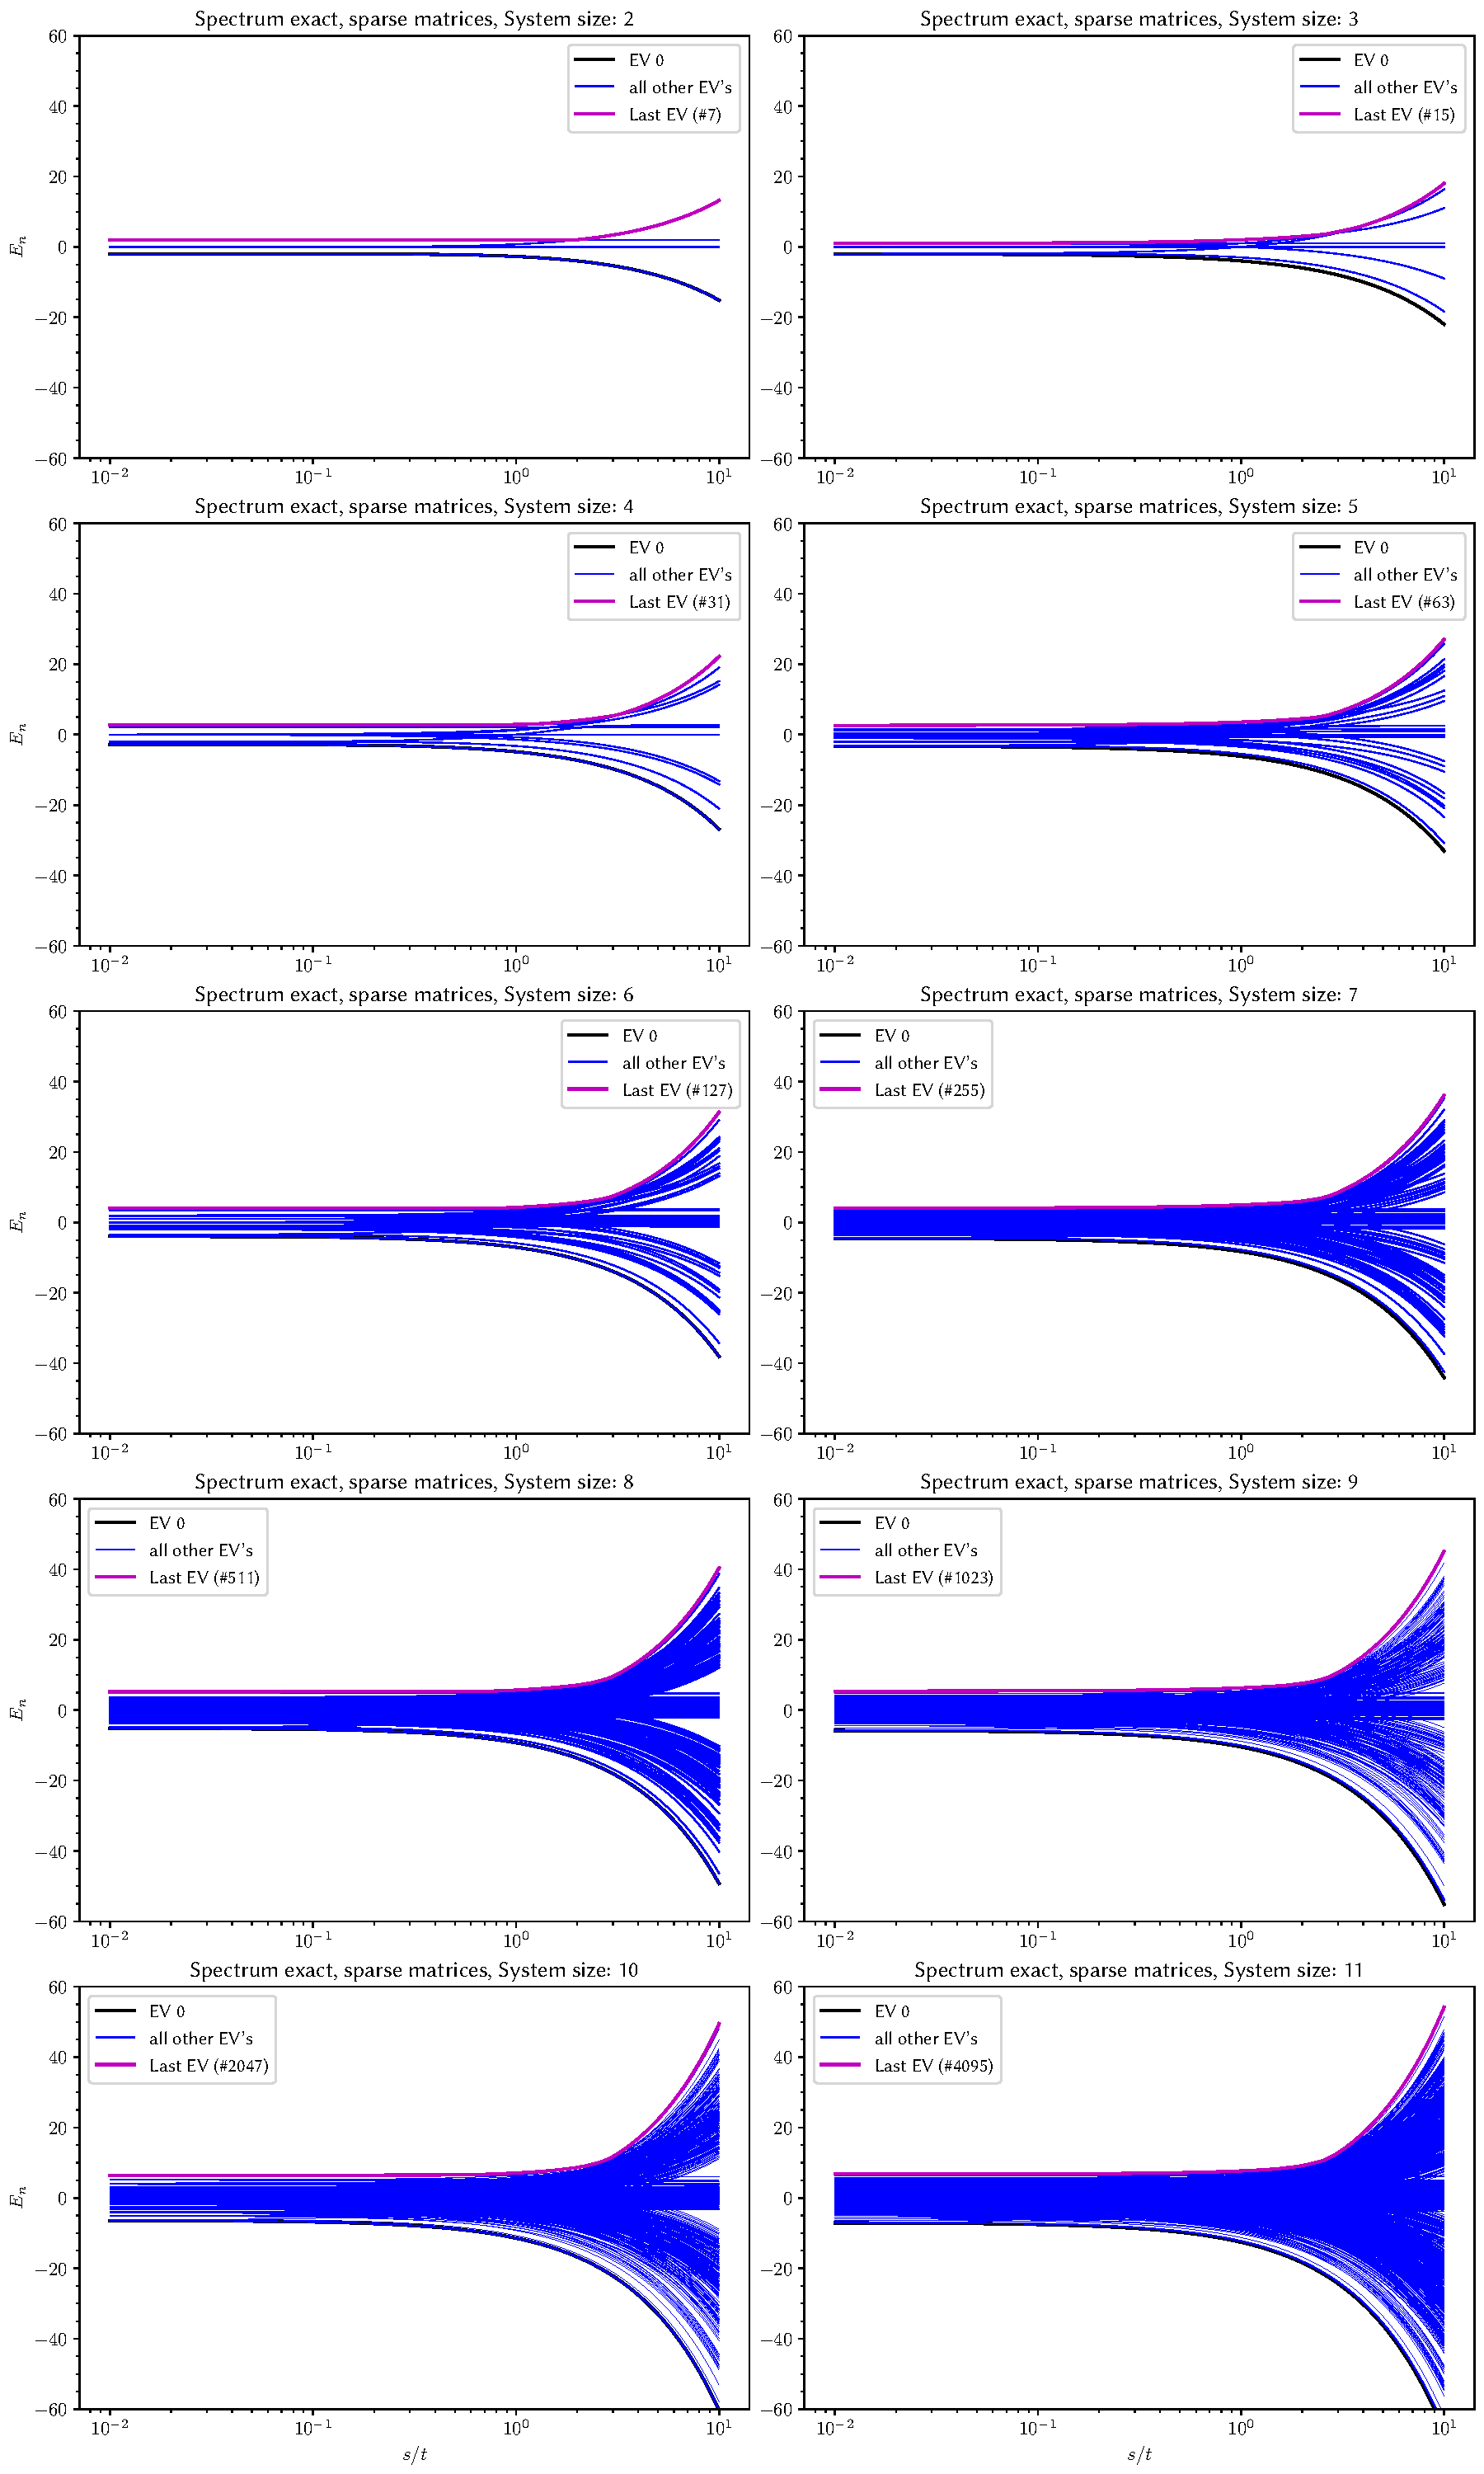
\includegraphics[width=\textwidth]{graphics/spectrum_exact.pdf}
        \caption{Spectrum of Hamiltonian for different system sizes}
        \label{fig:spectrum_exact}
    \end{figure}
    \clearpage

\subsection{Problem 1 (d)}
    \label{sec:d}
    
    To plot the condensate fraction, the Hamiltonian from Problem \ref{sec:b} and \ref{sec:c} is diagonalised again. Its ground state is easily picked as the eigenvector corresponding to the (algebraically) smallest (possibly negative) eigenvalue. The expectation value of the correlator matrix $C(i,j)$ from Problem \ref{sec:b} is then used to calculate the matrix elements of the reduced density matrix for the given $\nicefrac{s}{t}$ sample. 
    
    From the reduced density matrix, the largest eigenvalue $n_0$ corresponds to the largest number of particles that are correlated in the ground state.
    
    The trace $N$ is equivalent to the number of particles in the ground state, since the diagonal entries of the correlator are just the number operators of a site in the Fock space.
    \begin{align}
        N = \sum_j \bra{\psi_0}\hat{n}_j\ket{\psi_0}
    \end{align}
    $\rho := \frac{N}{L+1}$ is stored alongside the condensate fraction to store the filling level of the wheel. The condensation fraction is now plotted against $\frac{s}{t}$ in \autoref{fig:cond_frac}. The even and odd values of $L$ are separated to not crowd the plot. Additionally, the coloring is picked according to $\rho$, not $L$, since there are sometimes multiple trajectories visible for the same $L$.

    We observe that the condensation fractions increase in a sigmoid-like way with increasing $s/t$. In general, an increase in the condensation fraction for $\frac{s}{t} > 1$ makes sense. In this regime, the hardcore bosons prefer to hop to the center site, which is why they become increasingly correlated, since every site of the wheel is a neighbour to the center. This corresponds nicely with the regime in which the eigenvalues split in Problems \ref{fig:spectrum_manual} and \ref{fig:spectrum_exact}. As the ground state energy gets more negative (the ground state "gets cheaper"), the system's condensation rises. Globally, the even $L$ trajectories are at higher condensation fractions than the odd ones. The $L=2$ trajectory even stays constant at $1$, corresponding to a fully correlated system. Since $\rho = \nicefrac{1}{3}$ in this case, $N$ must equal $1$. Therefore there is only one particle occupying the ground state, which trivially correlates with itself, leading to a trivial condensation fraction.
            
    \begin{figure}[t!]
        \centering
        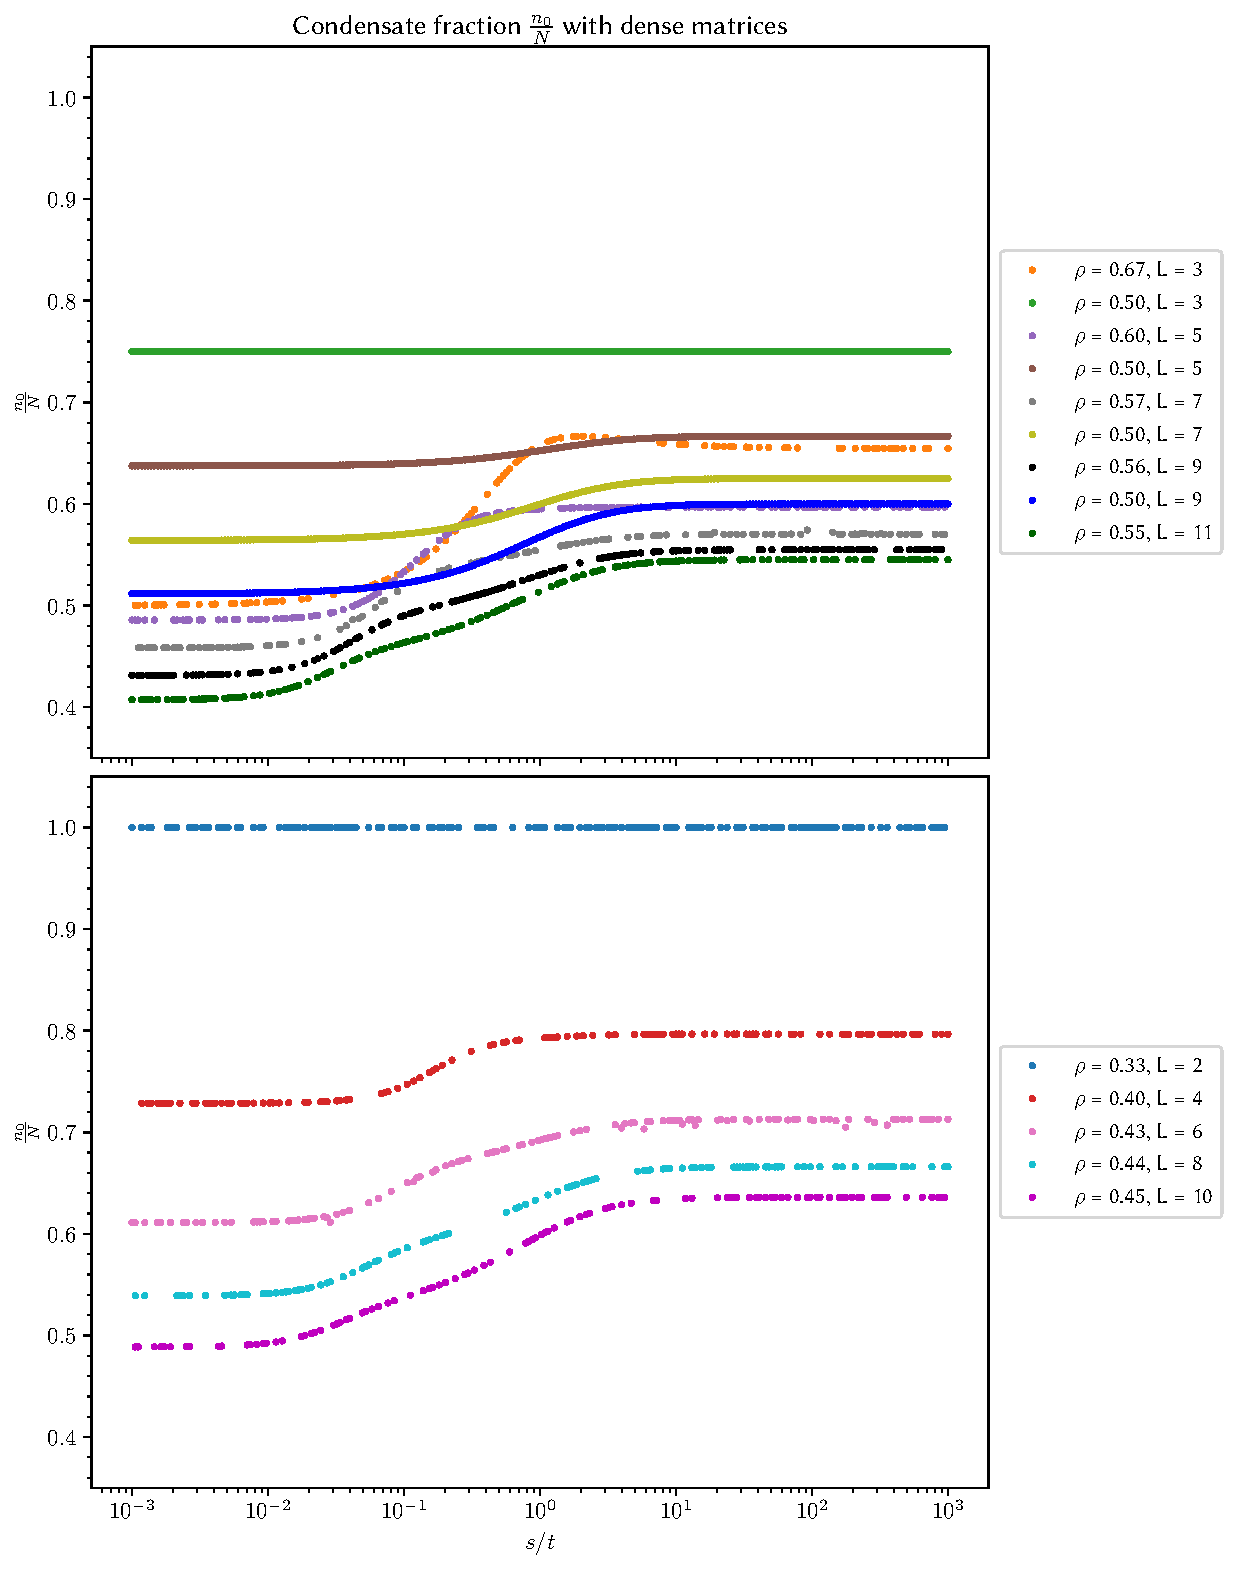
\includegraphics[width=\textwidth]{graphics/condensate_fraction.pdf}
        \caption{Condensate fractions for different number of sites and filling levels}
        \label{fig:cond_frac}
    \end{figure}
    
    We observed that all trajectories increase with growing $\nicefrac{s}{t}$ (except for tiny overshoots when settling into constant values and globally constant values). This effect is nicely illustrated on the last page in the supplementary material of \cite{wilkeSymmetryprotectedBoseEinsteinCondensation2022} in Figure S3. There, the fact that growing $s$ corresponds to higher condensate fractions is nicely illustrated across a wide range of system sizes.

    Note that the seemingly uninterrupted lines for $\rho = \nicefrac{1}{2}$ are just an artefact of the scatter plot marker size in combination with the given resolution in $\nicefrac{s}{t}$ and don't carry any physical significance.

    
\clearpage
\section{Conclusion and Areas for Improvement}
    In conclusion, we solved the eigenvalue problem for a system size up to $L = 11$ ($12$ lattice sites in total) in the time that we were given. Unfortunately, on the last day, we noticed an error in the code that meant that we had to rerun all the calculations. Due to time constraints, we were only able to solve for a system size up to $L = 10$ ($11$ lattice sites in total).

    Of course, given the short timeframe, the work done in this project could be improved in many ways, on top of what we have already mentioned within the text. 
    
    Firstly, the condensate fraction calculation could have been integrated with the spectrum calculation so that the same Hamiltonian need not be diagonalised twice. 
    
    Secondly, The \texttt{run.py} script could also have recorded the runtimes of each of the steps, which would have allowed us to visualise the scaling of the problem as a function of lattice size $L$. 

    Thirdly, the exact reason why the code does not run on the cluster could be further investigated so that one may have access to much larger computational resources.

    Last but not least, we could have also employed the Jordan-Wigner Transformation to reduce the complexity of the problem numerically \cite{wilkeSymmetryprotectedBoseEinsteinCondensation2022}. 

    

    
\printbibliography
\end{document}
